\id{ҒТАМР 81.93.29}{}

\begin{articleheader}
\sectionwithauthors{Б.Е. Ихсанова, Б. Бөрібаев, М.С. Сериккажина}{ЦИФРЛАНДЫРУ ЖАҒДАЙЫНДА ҰЙЫМДАРДЫҢ АҚПАРАТТЫҚ ҚАУІПСІЗДІК
САЯСАТЫНЫҢ ТИІМДІЛІГІН БАҒАЛАУДЫҢ ӘДІСТЕМЕЛІК ТӘСІЛДЕРІН ТАЛДАУ}

{\bfseries
Б.Е. Ихсанова\alink{https://orcid.org/0009-0007-9202-9650}\textsuperscript{\envelope },
Б. Бөрібаев\alink{https://orcid.org/0009-0004-8866-9581},
М.С. Сериккажина \alink{https://orcid.org/0009-0001-0280-3099}
}
\end{articleheader}

\begin{affiliation}
Әл-Фараби атындағы Қазақ Ұлттық Университеті, Алматы, Қазақстан

\raggedright \textsuperscript{\envelope }Корреспондент-автор: botagozikhsanova@gmail.com
\end{affiliation}

Экономика мен қоғамның қарқынды цифрлық дамуы жағдайында ұйымдардың
ақпараттық қауіпсіздігін қамтамасыз ету тұрақтылық пен бәсекеге
қабілеттіліктің негізгі факторы болып табылады. Ұйымдар деректердің
сыртқа шығуы, кибершабуылдар және рұқсатсыз қол жеткізу сияқты
қауіптердің күшеюімен бетпе-бет келеді. Мақала техникалық,
ұйымдастырушылық және әлеуметтік аспектілерді ескере отырып, ұйымдардағы
ақпараттық қауіпсіздік саясатының тиімділігін бағалаудың әдіснамалық
тәсілдерін талдауға арналған. Зерттеу барысында техникалық және
ұйымдастырушылық факторлар, сондай-ақ әлеуметтік-техникалық контекст
ескерілген. Халықаралық стандарттар (ISO/IEC 27001, NIST SP 800-53,
COBIT), сандық әдістер (FMEA, OCTAVE), мультикритериалды талдау (MCDA)
және киберқауіпсіздік жетілу модельдері талданып, олардың артықшылықтары
мен шектеулері анықталды. Әдістерді қолданудың тиімділігі ұйымның
құрылымы мен оның цифрлық инфрақұрылымының ерекшеліктеріне байланысты
өзгеретіні дәлелденді. Ғылыми зерттеулерге негізделген талдау құқықтық
реттеу, басқарушылық құрылым және ақпараттық активтерді техникалық
қорғау мәселелерін қамтыды. Эмпирикалық деректер негізінде бағалау
әдістерінің салыстырмалы талдауы жүргізіліп, олардың қолданылуында
кездесетін негізгі мәселелер анықталды. Зерттеу нәтижелеріне сүйене
отырып, ақпараттық қауіпсіздікті басқару жүйесін жетілдіру, ресурстарды
оңтайлы пайдалану және киберқауіптерге төзімділікті арттыру бойынша
ұсыныстар әзірленді. Жүргізілген зерттеу ақпараттық қауіпсіздікті
бағалауда жүйелі тәсілді қолданудың маңыздылығын растайды. Халықаралық
стандарттар, сандық көрсеткіштер және стратегиялық басқару әдістерін
біріктіру арқылы ұйымдар ықтимал қауіптерді төмендетіп, деректерді
қорғау деңгейін арттырып, кибершабуылдарға қарсы тұрақтылығын күшейте
алады.

{\bfseries Түйін сөздер:} ақпараттық қауіпсіздік саясаты, цифрландыру,
тиімділік, ақпараттық қауіпсіздік, әдістемелік тәсілдер,
киберқауіпсіздік, халықаралық стандарттар, кешенді талдау.

\begin{articleheader}
{\bfseries АНАЛИЗ МЕТОДИЧЕСКИХ ПОДХОДОВ К ОЦЕНКЕ ЭФФЕКТИВНОСТИ ПОЛИТИКИ
ИНФОРМАЦИОННОЙ БЕЗОПАСНОСТИ ОРГАНИЗАЦИЙ В УСЛОВИЯХ ЦИФРОВИЗАЦИИ}

{\bfseries
Б.Е. Ихсанова\textsuperscript{\envelope },
Б. Бөрібаев,
М.С. Сериккажина
}
\end{articleheader}

\begin{affiliation}
Казахский национальный университет имени аль-Фараби, Алматы, Казахстан,

e-mail: botagozikhsanova@gmail.com
\end{affiliation}

В условиях стремительного цифрового развития экономики и общества
обеспечение информационной безопасности организаций является ключевым
фактором устойчивости и конкурентоспособности. Организации сталкиваются
с растущими угрозами, такими как утечки данных, кибератаки и
несанкционированный доступ. Целью статьи является анализ методических
подходов к оценке эффективности политики обеспечения информационной
безопасности в организациях с учетом технических, организационных и
социальных аспектов. В исследовании учитывались технические и
организационные факторы, а также социально-технический контекст. Были
проанализированы международные стандарты (ISO/IEC 27001, NIST SP 800-53,
COBIT), количественные методы (FMEA, OCTAVE), многокритериальный анализ
(MCDA) и модели зрелости кибербезопасности, а также выявлены их
преимущества и ограничения. Доказано, что эффективность применения
методов различается в зависимости от структуры организации и
особенностей ее цифровой инфраструктуры. Анализ, основанный на научных
исследованиях, охватывал вопросы правового регулирования, структуры
управления и технической защиты информационных активов. На основе
эмпирических данных проведен сравнительный анализ методов оценки и
выявлены основные проблемы, возникающие при их применении. По
результатам исследования разработаны рекомендации по совершенствованию
системы управления информационной безопасностью, оптимизации
использования ресурсов и повышению устойчивости к киберугрозам.
Проведенное исследование подтверждает важность использования системного
подхода при оценке информационной безопасности. Интегрируя международные
стандарты, количественные показатели и методы стратегического
управления, организации могут снизить потенциальные угрозы, усилить
защиту данных и повысить устойчивость к кибератакам.

{\bfseries Ключевые слова:} политика информационной безопасности,
цифровизация, эффективность, информационная безопасность,
методологические подходы, кибербезопасность, международные стандарты,
комплексный анализ.

\begin{articleheader}
{\bfseries ANALYSIS OF METHODOLOGICAL APPROACHES TO ASSESS THE
EFFECTIVENESS OF ORGANIZATIONS'{} INFORMATION SECURITY
POLICIES IN THE CONTEXT OF DIGITIZATION}

{\bfseries
B.Ye. Ikhsanova\textsuperscript{\envelope },
B. Buribayev,
M.S. Serikkazhina
}
\end{articleheader}

\begin{affiliation}
Al-Farabi Kazakh National University, Almaty, Kazakhstan,

e-mail: botagozikhsanova@gmail.com
\end{affiliation}

In the context of the rapid digital development of the economy and
society, ensuring information security of organizations is a key factor
in their stability and competitiveness. Organizations are faced with
increasing threats such as data leakage, cyberattacks, and unauthorized
access. The article is devoted to the analysis of methodological
approaches to assessing the effectiveness of information security
policies in organizations, taking into account technical,
organizational, and social aspects. The study takes into account
technical and organizational factors, as well as the socio-technical
context. International standards (ISO/IEC 27001, NIST SP 800-53, COBIT),
quantitative methods (FMEA, OCTAVE), multi-criteria analysis (MCDA), and
cybersecurity maturity models are analyzed, and their advantages and
limitations are identified. It is proved that the effectiveness of the
methods varies depending on the structure of the organization and the
characteristics of its digital infrastructure. The analysis, based on
scientific research, covers issues of legal regulation, management
structure, and technical protection of information assets. Based on
empirical data, a comparative analysis of assessment methods was
conducted and the main problems encountered in their application were
identified. Based on the results of the study, recommendations were
developed to improve the information security management system,
optimize resource utilization, and increase resilience to cyber threats.
The study confirms the importance of using a systematic approach to
information security assessment. By combining international standards,
quantitative indicators, and strategic management meth\-ods, organizations
can reduce potential threats, increase the level of data protection, and
strengthen their resilience to cyber attacks.

{\bfseries Keywords:} information security policy, digitalization,
efficiency, information security, methodological approaches,
cybersecurity, international standards, comprehensive analysis.

\begin{multicols}{2}
{\bfseries Кіріспе.} Қазіргі кезеңде цифрлық технологиялар мен ақпараттық
жүйелер әртүрлі салалар мен ұйымдардың қызметінде елеулі орын алуда.
Ақпараттық ресурстарға тәуелділіктің өсуі деректердің құпиялылығы,
тұтастығы және қолжетімділігі мәселелеріне, сонымен қатар
киберқатерлерден туындайтын тәуекелдерді басқаруға ерекше назар аударуды
қажет етеді. Жаһандық цифрландыру жағдайында кибершабуылдар коммерциялық
және мемлекеттік құрылымдарға жиі әсер ететін құбылысқа айналды {[}1{]}.
Ақпараттық жүйелердің жеткілікті қорғалмауы немесе бекітілген
қауіпсіздік нормаларының сақталмауы құпия мәліметтердің таралуына,
технологиялық процестердің бұзылуына, қаржылық шығындарға және ұйымға
деген сенімнің төмендеуіне әкелуі ықтимал.

Қауіп-қатерлерге қарсы әрекет етудің түрлі әдістері ішінде ақпараттық
қауіпсіздік (АҚ) саясатын қалыптастыру мен бағалауда жүйелік амал аса
маңызды рөл атқарады. Мұндай саясат ақпаратты рұқсатсыз
қолжетімділіктен, өзгертуден және жоюдан қорғауға бағытталған нормалар,
ережелер, құралдар және ұйымдастырушылық шаралар жиынтығын реттейді.
Алайда практикада көптеген ұйымдарда қауіпсіздік шаралары тепе-теңдікте
енгізілмейді, олардың тиімділігін бағалау критерийлері нақты болмайды,
ал нақты тәуекелдер деңгейіне сәйкестігін талдауға арналған әдістемелік
тетіктер жеткіліксіз болып жатады. Технологиялық, адами және
басқарушылық аспектілерді ескеретін кешенді зерттеу қажеттілігі
туындайды {[}2{]}.

Зерттеу мақсаты - цифрландыру жағдайында ұйымдардың ақпараттық
қауіпсіздік саясатының тиімділігін бағалау бойынша методологиялық
амалдарды талдап, әртүрлі мемлекет ғалымдарының тәжірибесі мен
нормативтік-құқықтық базаны, заманауи халықаралық стандарттарды (NIST,
ISO/IEC 27001 және басқа) ескеріп қорытындылау.

Ақпараттық технологиялардың дамуы деректердің таралуымен және
кибершабуылдармен байланысты жаңа қатерлердің пайда болуына ықпал етіп,
тәуекелдерді бақылаудың маңыздылығын күшейтті. Қазақстан мен ТМД елдері
аясында ақпараттық қауіпсіздік мемлекеттік саясаттың басты бағыттарының
біріне айналды, мұны әртүрлі мемлекеттік бағдарламалар мен заңнамалық
актілер растайды. Байкенов Б.С. және Оразалиева С.К. {[}3{]} ұйымдардағы
қорғаныс қызметтерін ұйымдастыру мен басқару мәселелерін талдай келе,
құқықтық, техникалық және ұйымдастырушылық аспектілерді қамтитын кешенді
амалдың қажеттілігін атап өтеді. Ғалымдардың пайымдауынша, негізгі
қиындықтардың бірі -- бизнес-мақсаттармен өзара байланысты және
тәуекелдерді жүйелі түрде бағалауға негізделген қауіпсіздік шараларын
енгізудегі фрагменттік тәсіл.

Қазақстандағы нормативтік-құқықтық базаға келсек, министрліктердің
қаулылары мен бұйрықтарын қоса алғанда, АҚ саласындағы қызметті
реттейтін құжаттар бекітілген {[}4{]}. Атап айтқанда, №\,82 «Қазақстан
Республикасының Ұлттық экономика министрінің\ldots» (2021) құжаты ұлттық
қауіпсіздік стратегиясын әзірлеу және мониторинг жүргізу сұрақтарын
қамтиды, онда ақпараттық қауіпсіздікке де назар аударылады. Дегенмен іс
жүзінде бірізді стандарттардың болмауы, мемлекеттік органдар арасындағы
мәлімет алмасудың тиімсіздігі және персоналдың хабардарлығының төмендігі
сияқты бірқатар мәселе байқалады. Осы себепті ғылыми-зерттеу жұмыстары
мен қолданбалы шешімдер ұсынатын әдістемелік нұсқаулықтардың маңызы
артып отыр.

Халықаралық тәжірибе тұрғысынан Коста И. және Гуарда Т. {[}5{]} еңбегі
қызығушылық тудырады, онда FMEA (Failure Mode and Effects Analysis)
негізінде ақпараттық жүйелердегі тәуекелдерді даралаудың жаңа әдісі
сипатталады. Авторлар инженерия саласындағы ақауларды талдау құралдарын
IT-инфрақұрылымдағы осалдықтарды бағалауға бейімдеудің жолын көрсетеді.
Бұл тәсіл қатерлерді формалды түрде есептеп, басымдықтарды айқындауға,
сәйкесінше қауіпсіздік саясатын реттеуге мүмкіндік береді.

Құқықтық негіз бен АҚ саясаты Полякова Т.А., Минбалеева А.В. және
Бойченко И.С. {[}6{]} еңбегінде кең түрде зерттеледі. Авторлар жаһандық
ортада цифрлық технологияларды қауіпсіз пайдаланудың құқықтық қамтамасыз
етілуі мәселелерін қозғай отырып, желілерде қолжетімді деректердің
көбеюі киберқылмыс өрісін кеңейтетінін атап көрсетеді. Бұл мақаладағы
талданған тұжырымдар АҚ саясатын қалыптастыруда құқықтық тәуекелдерді де
қарастырудың маңызды екенін айғақтайды. Ғалымдардың айтуынша, техникалық
шаралармен (шифрлау жүйелері, брандмауэрлер және т.б.) шектелу
жеткіліксіз, ұйым ішінде заң талаптарын және корпоративтік
регламенттерді сақтау тетіктерін айқын реттеу керек.

Қазақстандық зерттеушілер Мейрамбек Ә., Думанқызы Ж., Жұман А. және
Марбек Т. {[}7{]} еңбектерінде ақпараттық қауіпсіздіктің маңызы мен
жекелеген кәсіпорындар деңгейінде туындайтын қатерлерге талдау жасалады.
Авторлар «әлеуметтік инженерия» түріндегі шабуылдардың көбеюіне,
қызметкерлердің қауіп-қатерлер жайлы сауаттылығының жеткіліксіздігіне
және жүйелі оқыту жұмыстарының кемшін екеніне назар аударады. Мұндай
жағдайда қауіпсіздік саясатын қалыптастыру мәселесі персоналды оқытып,
ақпараттық қорғанысты нығайту шараларымен тоғысады.

Техникалық тұрғыдан алғанда, желілік ортада ақпаратты қорғау әдістері
Шаньгин В. Ф. {[}8{]} монографиясында қарастырылған. Криптография,
бұзуларды анықтау жүйелері, тұтастықты қамтамасыз ету және рұқсаттарды
шектеу секілді құралдар сипатталады. Автор ақпараттық қауіпсіздікті
кешенді түрде жүзеге асыру үшін техникалық және әкімшілік шараларды
үндестіріп, тұрақты мониторинг пен аудит жасау қажеттігін айтады. Бұл
деректер кез келген қауіпсіздік саясатына техникалық негіздерді
үйлестірудің өзекті екенін көрсетеді. Али Р. Ф. {[}9{]} еңбегінде
ақпараттық қауіпсіздік саясатына сәйкестік және мінез-құлықтық
ерекшеліктер талқыланады. Ғалым ұйымдарда қауіпсіздік шараларының
тиімділігі персоналдың бейілділігі мен сауаттылығына тәуелді екенін
дәлелдейді. Қызметкерлердің тәртібін өзгерту, оқыту және мотивация
принциптерін енгізу қажеттігі адамға негізделген факторларды компанияның
АҚ стратегиясына қосу маңыздылығын көрсетеді. Разикин К. және Соэвито Б.
{[}10{]} ұйым ішіндегі қауіпсіздік жүйесін қалыптастыру үшін
тәуекелдерді талдауға негізделген шешім қабылдау үлгісін ұсынады.
Авторлардың айтуынша, қолданыстағы құралдар болғанымен, көптеген ұйымдар
адами факторды жете бағаламайды және саяси ережелерді орындауды қолдауға
бағытталған оқыту мен ынталандыру шаралары жеткілікті деңгейде
қолданылмайды.

Жүргізілген талдау ақпараттық қауіпсіздіктің күрделі, көпқырлы сипатқа
ие екенін растайды: АҚ тек технологиялық немесе құқықтық қырлармен
шектелмей, сонымен бірге ұйымдастырушылық, экономикалық және адами
факторларға да тәуелді. Тиімділікті бағалауға арналған әдістеменің
біртұтас әрі дәл болуы маңызды. Көптеген зерттеулер тәуекелдер, шығындар
және пайда арақатынасын салыстыруға мүмкіндік беретін анағұрлым
формалды, көпкритерийлі үлгілерді құрастыру үрдісін көрсетіп отыр.

{\bfseries Материалдар мен әдістер.} \emph{Талдау әдістері:}

- таңдалған әдебиеттердің контент-талдауы;

- ақ тиімділігін бағалаудың түрлі әдістемелерін салыстырмалы талдау
(сапалық және сандық, тәуекелге негізделген және бақылауға
негізделген);

- ақ саласында шешім қабылдауға ықпал ететін факторларды жүйелеу
(техникалық, құқықтық, ұйымдастырушылық, адами, экономикалық);

- критерийлер жиынтығына (тәуекелдер, шығындар, процестің жетілу
деңгейі, адам факторы) негізделген кешенді бағалау моделін ұсынудың
кешенді тәсілі.
{\bfseries Нәтижелер мен талқылау.} Зерттеу барысында ұйымдардың цифрлық
трансформация жағдайындағы ақпараттық қауіпсіздік саясатының тиімділігін
бағалауға арналған әдістемелік амалдарға салыстырмалы талдау жасалды.

Нәтижелер көрсеткендей, әдісті таңдау бірнеше факторға байланысты:
ұйымның АҚ саласындағы жетілу деңгейі, салалық ерекшелігі, қолжетімді
ресурстары және құқықтық талаптары. ISO/IEC 27001, COBIT, NIST сияқты
стандарттар, OCTAVE, FMEA сияқты сандық тәуекелдерді бағалау тәсілдері,
SCORING және сараптамалық сауалнама үлгілерін қамтитын қауіпсіздікті
басқару модельдері зерттелді. Әр әдістің артықшылықтары да, шектеулері
де бар. Мәселен, халықаралық стандарттар кешенді қамту деңгейін
қамтамасыз етіп, нормативтік талаптармен үйлеседі, бірақ тиімділікті
нақты есептейтін егжей-тегжейлі алгоритмдер әрдайым берілмейді. Ал
сандық әдістер объективті бағалауға қолайлы, дегенмен оларға дәл мәлімет
пен білікті мамандар қажет (1 кесте) {[}11{]}.

1 кестеде жүргізілген талдау бірыңғай мінсіз әдістің жоқ екенін
көрсетеді. Тәуекелдерді сандық бағалау қажет болғанда OCTAVE, FMEA,
AI/ML қолданылады. IT Governance құрылымына интеграция жасау көзделген
жағдайда ISO/IEC 27001 немесе COBIT тартымды болып келеді. ISO/IEC 27001
Annex A бөлімінде бірқатар бақылау шаралары қарастырылған, бірақ
тәуекелдерді бағалаудың егжей-тегжейлі алгоритмі берілмеген. COBIT - IT
Governance бойынша жалпы база, соның ішінде АҚ аспектілерін қамтиды.
OCTAVE (CERT әзірлеген) -- активтерді, қатерлерді және осалдықтарды
талдап, басымдықты айқындауды ұсынады. FMEA бастапқыда инженерлік
ақауларды болдырмау үшін қолданылған, кейін IT саласына бейімделген
{[}12{]}. NIST-- АҚШ және басқа елдерде кең тараған жүйе, Identify,
Protect, Detect, Respond, Recover функцияларын қамтиды. ML/AI
негізіндегі шешімдер үлкен деректерге сүйеніп, аномалияларды анықтауда
қолданылады, бірақ басқару практикасында әлі де қалыптасу үстінде.
SCORING -- ұйымдардың ішкі процедураларына бағытталып, адами факторды
ескеретін үлгілер тобы. Сараптамалық сауалнамалар -- бастапқы кезеңде
пайдалы, бірақ формалды оңтайландыруға келмейді. Кейбір ұйымдар
техникалық және ұйымдастырушылық қырларды қамту үшін бірнеше әдісті
үйлестіруді жөн санайды {[}13{]}.

Ұйымдардың ақпараттық қауіпсіздік саясатының тиімділігін талдау бес
негізгі сала бойынша жүргізілді:

- физикалық қауіпсіздік;

- техникалық қорғаныс;

- ақпараттық ресурстарды басқару;

- персоналды басқару;

- тәуекелдерді басқару.
1-суретте әр сала бойынша бағалау көрсеткіштері берілген.
\end{multicols}

\tcap{1 - кесте. Ақпараттық қауіпсіздік саясатының тиімділігін бағалауға арналған әдістемелік амалдарды салыстырмалы талдау}
\begin{longtblr}[
  label = none,
  entry = none,
]{
  width = \linewidth,
  colspec = {Q[121]Q[121]Q[127]Q[158]Q[175]Q[233]},
  rows = {font=\footnotesize},
  cells = {c},
  hlines,
  vlines,
}
Тәсіл & {Бағалау түрі (сапалық/ \\сандық)} & Басымдық
			(тәуекел / бақылау) & Метрикалар
			немесе KPI & Артықшыл\-ықтары & Шектеулері\\
1.
			ISO/IEC 27001 & Сапалық
			/ ішінара сандық & {Теңгерімді (тәуекел \\+бақылау)} & Жалпы:
			инцидент саны, сәйкестік пайызы \% & Халықаралық
			ауқым, жүйелік қамту & Нақты
			өлшемдерді таңдаудың ресми алгоритмін
			қамтамасыз етпейді\\
2.
			COBIT & Сапалық / жетілу деңгейі үлгісі & {Бақылау \\+ процестер} & Жетілудің
			деңгейлері & IT-басқаруды
			кеңінен қамтиды & Негізгі
			фокус тек АҚ-те емес\\
3.
			OCTAVE & Жартылай
			сандық & Тәуекелге
			бағытталған & Тәуекелдердің
			сандық индексі & Тәуекелді
			талдаудың егжей-тегжейлі сипаттамасы & Шағын
			ұйымдар үшін тым күрделі болуы мүмкін\\
4.
			FMEA & Сандық & Тәуекелге
			негізделген & RPN
			(Risk Priority Number) & Сандық
			көрсеткіштер нақты анықталады & Ақаулар
			ықтималдығын сипаттайтын деректердің
			толық болуы шарт\\
5.
			NIST Cyber\-security Framework & Сапалық / жетілу
			шкалалары & {Тәуекел \\+ бақылау} & Категориялар
			мен жетілу деңгейлері & Әмбебап
			үлгі, оны бейімдеу жеңіл & Жергілікті
			нормалармен сәйкес келмеуі мүмкін\\
6.
			ML/AI-based әдістер & Сандық / зияткерлік
			талдау & Тәуекел,
			аномалиялар & Аномалия
			белсенділігінің көрсеткіштері & Жаңа
			қатерлерге икемді икемделу & Деректер
			жиыны сапалы болуын талап етеді,
			әзірлеу күрделі\\
7.
			SCORING (авторлық әдістер) & Әртүрлі
			метрикалар & {Бақылау \\+ тәуекел} & Персоналдың
			тәртібін бағалау & Адами
			аспектіні қамтиды & Жалпыға
			ортақ есептеу стандарты жоқ, әр
			компанияға бейімдеу қажет\\
8.
			Сараптамалық сауалнама & Сапалық & Шартты
			(модельсіз) & Балдық
			бағалау & Қолдануға
			оңай & Субъективтілігі
			жоғары, басымдықты нақты бөлетін
			құралдар шектеулі
\end{longtblr}

\begin{figure}[H]
	\centering
	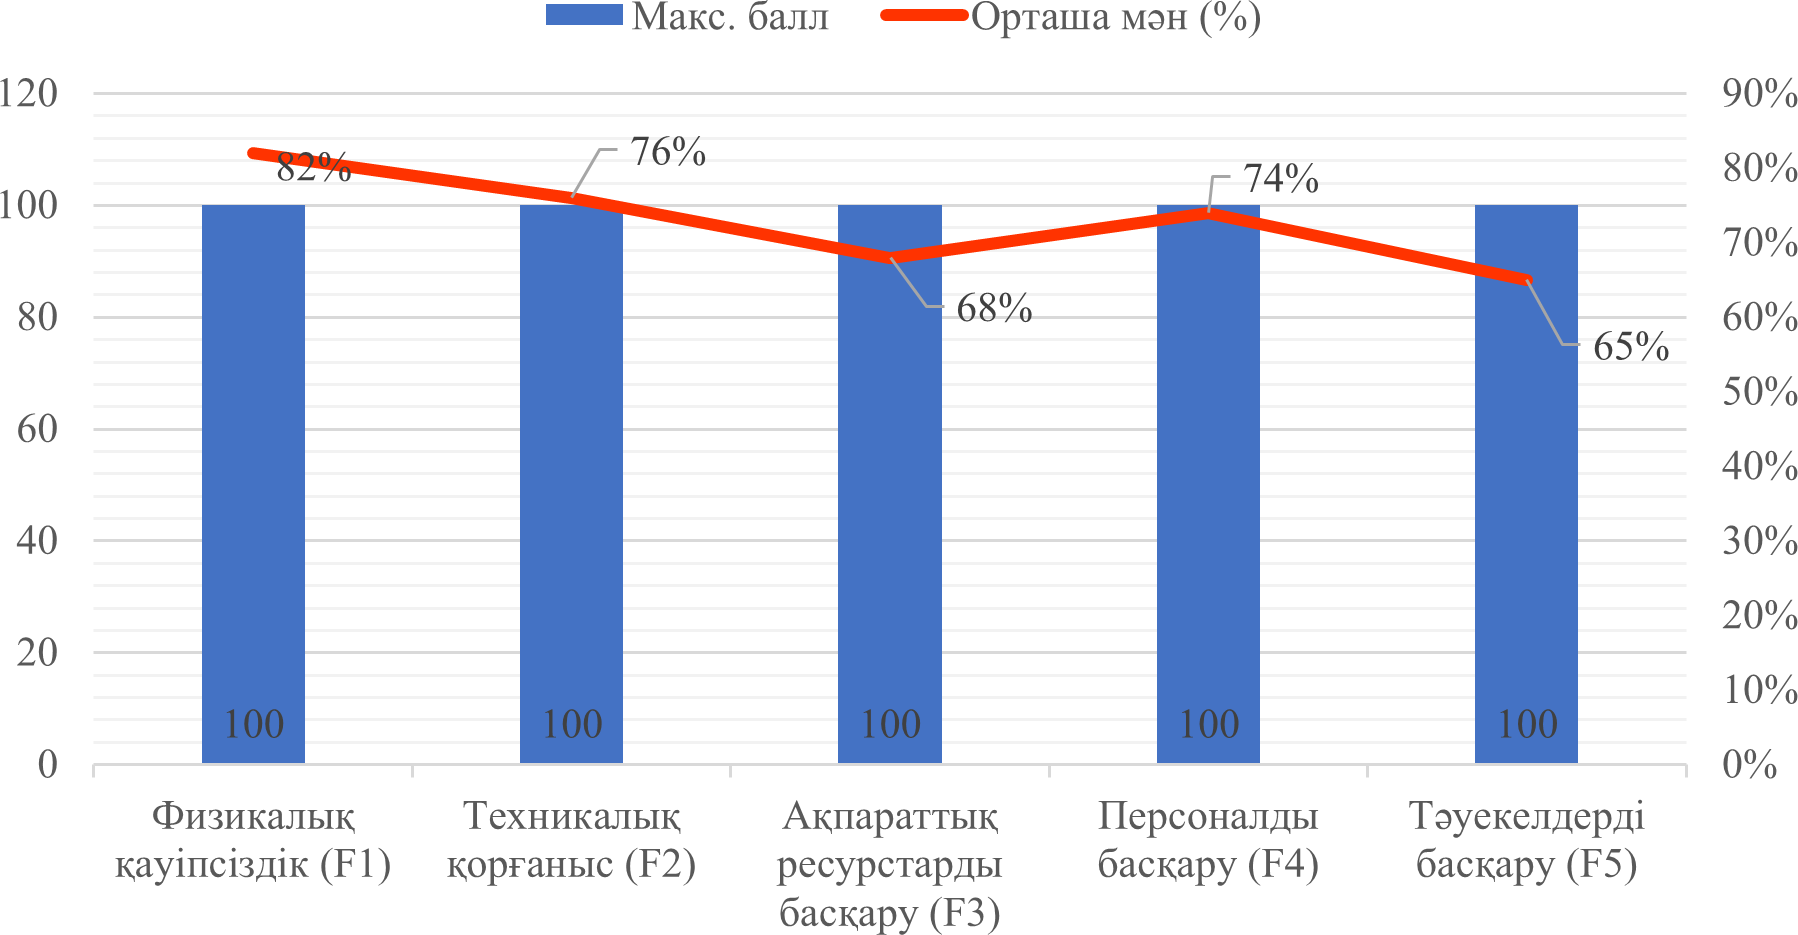
\includegraphics[width=0.8\textwidth]{media/ict4/image1}
	\caption*{1 - сурет. Ақпараттық қауіпсіздік саясатының тиімділігін бағалау}
\end{figure}

\begin{multicols}{2}
1 - суретте ақпараттық қауіпсіздіктің бес негізгі бағытының салыстырмалы
талдауының нәтижелері көрсетілген. Физикалық және техникалық
қауіпсіздіктегі жоғары көрсеткіштер инфрақұрылымды қорғауды қамтамасыз
етудегі жүйелі тәсілді көрсетеді, бірақ ақпараттық ресурстар мен
тәуекелдерді басқарудағы әлсіз көрсеткіштер ерекше назар аударуды қажет
етеді {[}14{]}.
\end{multicols}

\tcap{2 - кесте. Ақпараттық қауіпсіздік саясатының тиімділігіне әсер ететін негізгі факторлар}
\begin{longtblr}[
  label = none,
  entry = none,
]{
  width = \linewidth,
  colspec = {Q[133]Q[248]Q[144]Q[71]Q[108]Q[233]},
  rows = {font=\footnotesize},
  cells = {c},
  hlines,
  vlines,
}
Фактор & Сипаттамасы & Метрика
			мысалы & Ықпал
			деңгейі & Ресурстар & Ұсыныстар\\
1.Технология\-лық
			инфрақұрылым & Заманауи
			қорғаныс жүйелерін, антивирустарды,
			брандмауэрлерді, IDS/IPS пайдалануы & Негізгі
			IT-сегменттерді қамту пайызы & Жоғары & Лицензия\-лар,
			жабдық & Инфрақұрылымды
			жаңарту, аудит жүргізу\\
2.
			Құқықтық реттеу & Заңнамалық,
			салалық регламенттерді сақтауы & Бұзушылықтар
			/ айыппұлдар саны & Жоғары & Заң
			бөлімі & Комплаенс
			бөлімін құру, нормативтерді қадағалау\\
3.
			Персонал мәдениеті & Хабардарлық,
			тәртіп, АҚ саясатын орындаудағы ынтасы & Оқыту
			деңгейі (сауалнамалар) & Маңызды & Тренинг,
			HR & Тұрақты
			оқыту, марапаттау, тестілеу\\
4.
			Басқарушылық қолдау & Басшылықтың
			қатысуы, бюджет бөлу, басымдық беру & Жылдық
			қаржыландыру көлемі & Маңызды & Менеджмент,
			қаржы & Қажетті
			ресурстарды жеткілікті бөлу, KPI енгізу\\
5.
			Тәуекел-менеджмент & Тәуекелдерді
			анықтау, бағалау және өңдеу жүйесі & Кешіктірілген
			тәуекелдер саны, Risk Level & Жоғары & АҚ
			мамандары, жобалар & Тәуекелдерді
			тұрақты қайта бағалау, автоматтандыру\\
6.
			Ұйымдастырушылық құрылым & Рөлдер,
			жауапты тұлғалар және өкілеттіктердің
			айқын бөлінуі & Ұйымдық
			жетілу индексі (maturity) & Орташа & Ұйым
			сызбасы, регламенттер & Регламенттерді
			жаңарту, жауапты тұлғаларды тағайындау\\
7.
			Қаржы-экономикалық факторлар & Қорғаныс
			шараларының құны, жобалардың ROI, тәуекел
			мен пайданы салыстыру & ИБ
			жобаларының ROI, TCO & Жоғары & Қаржы
			бөлімі & Шығындарды
			оңтайландыру, басымдықтарды нақты
			көрсеткіштер бойынша түзу
\end{longtblr}

\begin{multicols}{2}
2 - кестеде ақпараттық қауіпсіздік саясатының табыстылығының негізгі
драйверлері адам факторы мен басқаруды қолдау болып табылатынын
көрсетеді, онсыз ешқандай техникалық шаралар жеткілікті тиімді болмайды.
Бұдан басқа, құқықтық реттеу және тәуекелдерді басқару нақты қорғау
әдістерін таңдау үшін «негіздерді» белгілейді.

Ақпараттық қауіпсіздікті бағалау бойынша заманауи зерттеулерде ISO/IEC
27001, NIST SP 800-53 және COBIT 5 сияқты халықаралық стандарттар
кеңінен қолданылады. Салыстырмалы талдауды көрсету үшін келесі диаграмма
құрастырылды (2-сурет).
\end{multicols}

\begin{figure}[H]
	\centering
	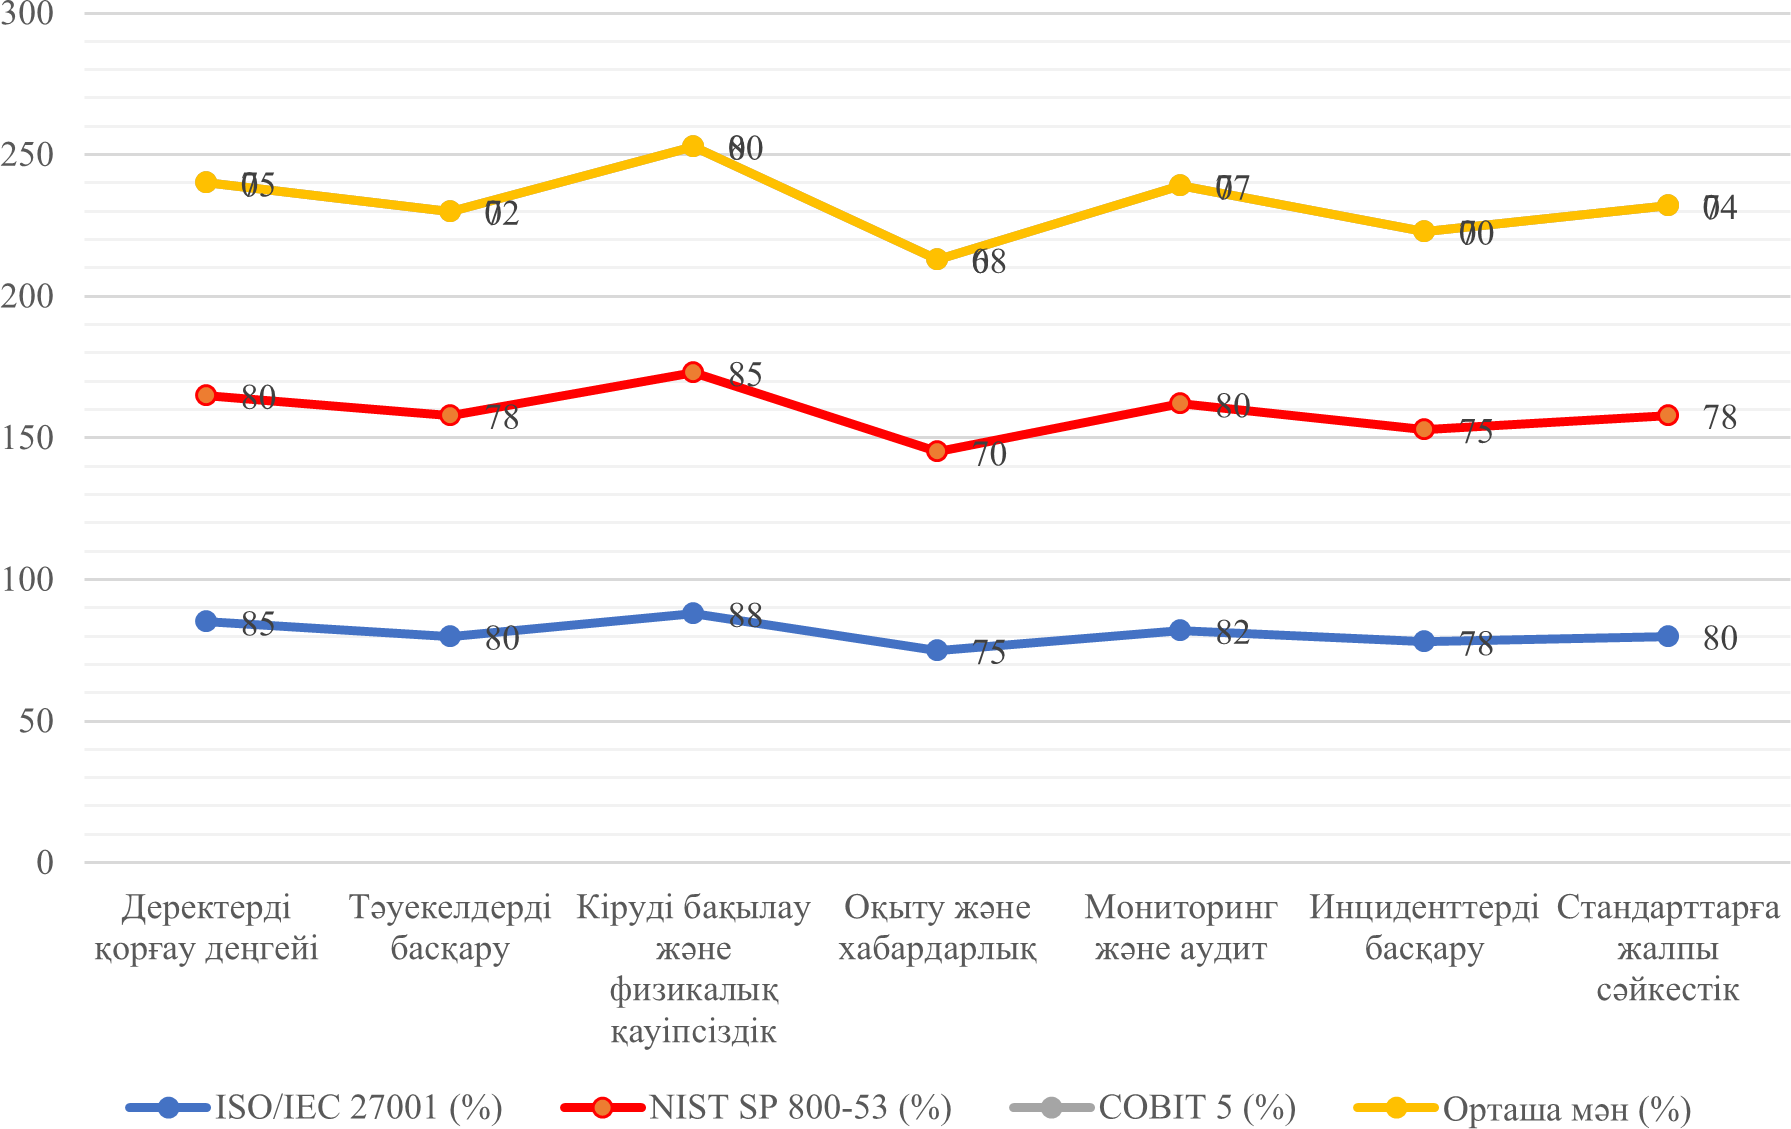
\includegraphics[width=0.8\textwidth]{media/ict4/image2}
	\caption*{2 - сурет. Ақпараттық қауіпсіздік стандарттарын енгізуді
салыстырмалы талдау}
\end{figure}

\begin{multicols}{2}
2 суреттегі зерттеу ISO/IEC 27001 және NIST SP 800-53 көптеген
көрсеткіштер бойынша COBIT 5-пен салыстырғанда жоғары орындау
жылдамдығын көрсететінін көрсетеді. Деректерді қорғау метрикасының
орташа мәні 80\% құрайды, бұл ұйымдарда техникалық шаралардың сенімді
орындалуын көрсетеді. Дегенмен, тәуекелдер мен оқиғаларды басқару
мәселелері өзекті болып қала береді, бұл әдістерді қосымша
оңтайландыруды және бейімдеуді талап етеді.

Салыстырмалы талдау ISO/IEC 27001 және NIST SP 800-53 сияқты халықаралық
стандарттарды қолдану COBIT 5-пен салыстырғанда техникалық шараларды
жүзеге асырудың жоғары деңгейіне ықпал ететінін көрсетеді. Дегенмен,
әмбебап стандарттар жергілікті жағдайларға бейімделуді талап етеді, бұл
«Стандарттарға жалпы сәйкестік» санатындағы төмен баллдармен расталады
(77,3\%). Бұл жекелеген ұйымдардың ерекшеліктері мен аймақтық
сипаттамалар аясында стандарттарды одан әрі бейімдеу және түсіндіру
қажеттілігін көрсетеді {[}15{]}.

Интеграциялық амал. Жинақталған деректер тиімділікті арттыру үшін
бірнеше құралды ұштастыруды маңызды санайды: тәуекелдерді сандық бағалау
(OCTAVE, FMEA), халықаралық стандарттарды орындау (ISO/IEC 27001, NIST)
және ұйымдастырушылық-басқарушылық шараларды енгізу (оқыту, мотивация,
бірыңғай регламенттер).

Икемділік. Цифрландыру қарқынының жеделдеуі жаңа технологиялар
(машиналық оқыту), шабуыл түрлері (фишинг, ботнет, жасырын майнерлер)
және заңнамалық өзгерістерді назарға алатын бейімделгіш саясатты талап
етеді.

Адам факторы. Персоналдың қауіпсіздік талаптарына сәйкес іс-әрекеті
маңызды орын иеленеді. Қызметкерлердің білім деңгейі жеткіліксіз болса,
ең заманауи техникалық құралдың өзі толық тиімділікке жеткізбейді.

Экономикалық қыр. Қорғаныс шараларын іске асыру шығындармен байланысты,
ал басшылық тәуекел мен бюджет арасында тепе-теңдік ұстанады. Саясаттың
пайдалылығын өлшеу үшін ROI, TCO сияқты көрсеткіштер қолданылады.

Осылайша, талдау нәтижелері әдістемелік тәсілдер әрқайсысының тиімді
жақтарын біріктіре отырып, кешенді түрде қолданылуы керектігін және
ұйымдардың өздері ұйымдастырушылық, экономикалық және адами аспектілерді
ескеруі қажет екенін растайды. Бұл тәуекелдерді формальды талдау,
стандарттарға сәйкестік және адам факторлары мен экономикалық
шектеулердің мониторингі нәтижелерін біріктіретін жүйелі бағалаудың
маңыздылығын көрсетеді.

{\bfseries Қорытынды.} Зерттеу негіздеріне сүйене отырып, жылдам
цифрландыру жағдайында ұйымның ақпараттық қауіпсіздік саясатының
тиімділігі технологиялық, құқықтық, ұйымдастырушылық және экономикалық
факторлардың жиынтығымен анықталады деген қорытындыға келуге болады.

Тәуекелдерді формальды талдауды (OCTAVE, FMEA), халықаралық
стандарттарды (ISO/IEC 27001, NIST), ұйымдастыру шараларын (персоналды
оқыту, заң талаптарын сақтау) және экономикалық есептеулерді (ROI, TCO)
қамтитын пәнаралық тәсілді қолдану қауіпсіздік саясатының тиімділігін
айтарлықтай арттыруы мүмкін. Басқарудың белсенділігі, қызметкерлер
арасындағы ақпараттық қауіпсіздік мәдениеті және тез өзгеретін
қауіптерге бейімделу сияқты аспектілер ерекше маңызды болып табылады.

Ақпараттық қауіпсіздік саясатының тиімділігіне әсер ететін негізгі
факторларға басшылықты қолдау, қызметкерлерді тарту, тәуекелдерді
басқару жүйесінің жетілуі, нормативтік талаптарға сәйкестік деңгейі және
қорғау шараларының экономикалық орындылығы екені анықталды. Зерттеу
сонымен қатар динамикалық өзгеретін киберқауіпті ортада ақпараттық
қауіпсіздік саясаты икемді және бейімделгіш болуы керек екенін көрсетті.
Тәуекелдердің тұрақты мониторингі, болжамды аналитикалық құралдарды
пайдалану және жасанды интеллектті қауіпсіздік процестеріне біріктіру
ұйымның қауіпсіздік деңгейін арттыруы мүмкін. Ақпараттық қауіпсіздікті
басқарудың қолданыстағы үлгілерін талдау барысында формальды
стандарттарды, сандық және сапалық бағалау әдістерін, сондай-ақ адам
факторын басқаруды біріктіретін интеграцияланған тәсілдерді қолданатын
ұйымдар ең табысты ұйымдар екені анықталды.

Осылайша, деректерге сүйене отырып, келесі ұсыныстарды жасауға болады:

- кадр әлеуетін күшейту: ақпараттық қауіпсіздік саласы бойынша
мамандарды тұрақты түрде оқыту, біліктілігін арттыру, ұйым ішінде
жауапкершілік мәдениетін қалыптастыру;

- формалды әдістерді біріктіру: NIST, ISO/IEC 27001 сияқты жүйелерді
AI/ML құралдарымен ұштастыру, тәуекелдер мен бақылау көрсеткіштерін
көпкритерийлі модельдер арқылы салыстыру;

- ұйымдастырушылық қолдау: жауапты құрылымдар мен өкілетті тұлғаларды
айқындау, ішкі регламенттер әзірлеу, аудит пен мониторинг процестерін
жиі жүргізу;

- экономикалық тиімділік: енгізілетін қорғаныс шараларының шығыны мен
пайдасын салыстыру, ROI, TCO әдістерін қолдану, ресурстарды оңтайлы
бөлу.
Зерттеу нәтижелері ақпараттық қауіпсіздік саясатының тиімділігі формалды
стандарттарды, тәуекел-менеджментті, басқару мәдениетін, заңды
жауапкершілікті және экономикалық орындылықты қамтитын кешенді амал
арқылы қамтамасыз етілетінін көрсетті. Цифрлық кеңістіктегі қатерлердің
күшеюі ұйымдарды қауіпсіздік жүйелерін икемді түрде жетілдіруге
жетелейді, бұл әлеуетті оқиғаларға төзімділікті арттыруға жол ашады.
\end{multicols}

\begin{center}
{\bfseries Әдебиеттер}
\end{center}

\begin{references}
1. Cabrera J.S., Reyes A.R.L., Lasco C.A. Multicriteria Decision Analysis
on Information Security Policy: A Prioritization Approach // Advanced
Technologies and Innovation. -- 2021. -Vol.6(1).- P.31-38. DOI
10.46604/aiti.2021.5476.

2. Сиротский А.А., Резниченко С.А. Формализованная модель аудита
информационной безопасности организации на предмет соответствия
требованиям стандартов // Безопасность информационных
технологий.-2021.-Т.28(3).- С.103-117. DOI 10.26583/bit.2021.3.09.

3. Байкенов Б.С., Оразалиева С.К. Ақпарат қауіпсіздігі мен қорғаныс
қызметін ұйымдастыру және басқару: оқу құралы. - Алматы: АЭжБУ, 2014. -
68 б. ISBN 6978-601-7327-50-7.

4. Қазақстан Республикасы Ұлттық экономика министрінің «Қазақстан
Республикасының Ұлттық қауіпсіздік стратегиясын әзірлеу, мониторингтеу,
іске асыру, бағалау және бақылау жүргізу әдістемесін бекіту туралы» 2021
жылғы 1 қыркүйектегі № 82 бұйрығы. URL:
\href{https://adilet.zan.kz/kaz/docs/V2100024227}{}
- Жүгінген күні: 09.01.2024.

5. Costa I., Guarda T. Information System Security Risk Priority Number:
A New Method for Evaluating and Prioritization Security Risk in
Information System Applying FMEA //Proceedings of International
Conference on Information Technology and Applications: ICITA 2021. --
Singapore : Springer Nature Singapore, 2022.-P.561-572. DOI
10.1007/978-981-16-7618- 5-49

6. Полякова Т. А., Минбалеев А. В., Бойченко И. С. Проблемы правового
обеспечения в информационной безопасности в процессе использования
цифровых технологий в глобальной цифровой среде// Вестник Академии права
и управления. - 2018. - №.3 (52). -- С.32-36.

7. Мейрамбек Ә., Думанқызы Ж., Жұман А., Марбек, Т. (2024). Ақпараттық
қауіпсіздіктің маңызы // Proceedings of the15thInternational Scientific
and Practical Conference «Scientific Horizon in the Context of Social
Crises» (April 26-28, 2024). Tokyo, Japan- Б.462--468

\href{https://doi.org/10.3390/app1108333}{}

8. Шаньгин, В. Ф. Информационная безопасность. -- Москва: ДМК Пресс,
2014. -- 702 c. -- ISBN 978-5-94074-768-0.

9. Ali R. F., Dominic P. D. D., Ali S. E. A., Rehman M., Sohail, A.
Information Security Behavior and Information Security Policy
Compliance: A Systematic Literature Review for Identifying the\\
Transformation Process from Noncompliance to Compliance // Applied
Sciences. - 2021. - Vol.11:3383.
\href{https://doi.org/10.3390/app11083383}{}

10. Razikin K., Soewito B. Cybersecurity decision support model to
designing information technology security system based on risk analysis
and cybersecurity framework //Egyptian Informatics Journal.
-2022.-Vol.23(3). - P.383-404.
\href{https://doi.org/10.1016/j.eij.2022.03.001}{}

11. Diéguez, M.; Bustos, J.; Cares, C. Mapping the variations for
implementing information security controls to their operational research
solutions//Inf. Syst.-Bus. Manage.- 2020.-Vol.18.-P.157-186.
~\href{https://doi.org/10.1007/s10257-020-00470-8}{}

12. Камалов Б. Р., Тумбинская М. В. Программное обеспечение для
обнаружения «скрытых майнеров» в браузерной среде // Прикладная
информатика.- 2023.-Т.18(1).- С.96-110.
\href{\%20https:/doi.org/10.37791/2687-0649-2023-18-1-96-110}{}

13. Мусабаев Р., Касымжанов Б., Калиева Г., Ибраева, В. Разработка
информационных технологий и систем для стимулирования устойчивого
развития личности как одна из основ развития Цифрового
Казахстана//Проблемы оптимизации сложных систем.-- 2018. - С.39-46.

14. Aldoseri A., Al-Khalifa K. N., Hamouda A. M. Methodological approach
to assessing the current state of organizations for AI-Based digital
transformation //Applied System Innovation. -2024.- Vol.7(1). - P.14.
\href{https://doi.org/10.3390/asi7010014}{}

15. Козырь Н. С., Оганесян Л. Л. Экономические аспекты информационной
безопасности: учебник и практикум для вузов. -- Москва:
Издательство~Юрайт, 2025. - 131 с. ISBN 978-5-534-17863-0
\href{https://urait.ru/bcode/568708}{}~-
Дата обращения:13.01.2025.
\end{references}

\begin{center}
{\bfseries References}
\end{center}

\begin{references}
1. Cabrera J.S., Reyes A.R.L., Lasco C.A. Multicriteria Decision Analysis
on Information Security Policy: A Prioritization Approach // Advanced
Technologies and Innovation. -- 2021. -Vol.6(1).- P.31-38. DOI
10.46604/aiti.2021.5476.

2. Sirotskij A.A., Reznichenko S.A. Formalizovannaja
model'{} audita informacionnoj bezopasnosti \\organizacii
na predmet sootvetstvija trebovanijam standartov //
Bezopasnost'{} informacionnyh tehnologij.-2021.-T.28(3).-
S.103-117. DOI 10.26583/bit.2021.3.09.{[}in Russian{]}

3. Bajkenov B.S., Orazalieva S.K. Aқparat қauіpsіzdіgі men қorғanys
қyzmetіn ұjymdastyru zhәne basқaru: oқu құraly. - Almaty: AJezhBU, 2014.
- 68 b. ISBN 6978-601-7327-50-7.{[}in Kazakh{]}

4. Қazaқstan Respublikasy Ұlttyқ jekonomika ministrіnің «Қazaқstan
Respublikasynyң Ұlttyқ қauіpsіzdіk strategijasyn әzіrleu, monitoringteu,
іske asyru, baғalau zhәne baқylau zhүrgіzu әdіstemesіn bekіtu turaly»
2021 zhylғy 1 қyrkүjektegі № 82 bұjryғy. URL:
https://adilet.zan.kz/kaz/docs/V2100024227 - Zhүgіngen kүnі: 09.01.2024.
{[}in Kazakh{]}

5. Costa I., Guarda T. Information System Security Risk Priority Number:
A New Method for Evaluating and Prioritization Security Risk in
Information System Applying FMEA //Proceedings of International
Conference on Information Technology and Applications: ICITA 2021. --
Singapore : Springer Nature Singapore, 2022.-P.561-572. DOI
10.1007/978-981-16-7618- 5-49

6. Poljakova T. A., Minbaleev A. V., Bojchenko I. S. Problemy pravovogo
obespechenija v informacionnoj bezopasnosti v processe
ispol' zovanija cifrovyh tehnologij v
global' noj cifrovoj srede// Vestnik Akademii prava i
upravlenija. - 2018. - №.3 (52). -- S.32-36. {[}in Russian{]}

7. Mejrambek Ә., Dumanқyzy Zh., Zhұman A., Marbek, T. (2024). Aқparattyқ
қauіpsіzdіktің maңyzy // Proceedings of the15thInternational Scientific
and Practical Conference «Scientific Horizon in the Context of Social
Crises» (April 26-28, 2024). Tokyo, Japan- B.462--468
DOI 10.51582/interconf.2024.198/{[}in Kazakh{]}

8. Shan' gin, V. F. Informacionnaja
bezopasnost'. -- Moskva: DMK Press, 2014. -- 702 c. --
ISBN 978-5-94074-768-0. {[}in Russian{]}

9. Ali R. F., Dominic P. D. D., Ali S. E. A., Rehman M., Sohail, A.
Information Security Behavior and Information Security Policy
Compliance: A Systematic Literature Review for Identifying the\\
Transformation Process from Noncompliance to Compliance // Applied
Sciences. - 2021. - Vol.11:3383.
\href{https://doi.org/10.3390/app11083383}{}

10. Razikin K., Soewito B. Cybersecurity decision support model to
designing information technology security system based on risk analysis
and cybersecurity framework //Egyptian Informatics Journal.
-2022.-Vol.23(3). - P.383-404.
\href{https://doi.org/10.1016/j.eij.2022.03.001}{}

11. Diéguez, M.; Bustos, J.; Cares, C. Mapping the variations for
implementing information security controls to their operational research
solutions//Inf. Syst.-Bus. Manage.- 2020.-Vol.18.-P.157-186.
~\href{https://doi.org/10.1007/s10257-020-00470-8}{}

12. Kamalov B. R., Tumbinskaja M. V. Programmnoe obespechenie dlja
obnaruzhenija «skrytyh majnerov» v brauzernoj srede // Prikladnaja
informatika.- 2023.-T.18(1).- S.96-110. DOI
10.37791/2687-0649-2023-18-1-96-110. {[}in Russian{]}

13. Musabaev R., Kasymzhanov B., Kalieva G., Ibraeva, V. Razrabotka
informacionnyh tehnologij i sistem dlja stimulirovanija ustojchivogo
razvitija lichnosti kak odna iz osnov razvitija Cifrovogo
Kazahstana // Problemy optimizacii slozhnyh sistem.-2018. - S.39-46.
{[}in Russian{]}

14. Aldoseri A., Al-Khalifa K. N., Hamouda A. M. Methodological approach
to assessing the current state of organizations for AI-Based digital
transformation //Applied System Innovation. -2024.- Vol.7(1). - P.14.
\href{https://doi.org/10.3390/asi7010014}{}

15. Kozyr'{} N. S., Oganesjan L. L. Jekonomicheskie
aspekty informacionnoj bezopasnosti: uchebnik i praktikum dlja vuzov. --
Moskva: Izdatel' stvo Jurajt, 2025. - 131 s. ISBN
978-5-534-17863-0 \href{https://urait.ru/bcode/568708}{https://urait.ru} - Data
obrashhenija:13.01.2025. {[}in Russian{]}
\end{references}

\begin{authorinfo}
\emph{{\bfseries Авторлар туралы мәліметтер}}

Ихсанова Б.Т.- «Ақпараттық технологиялар» факультетінің магистранты,
«Әл-Фараби атындағы Қазақ Ұлттық Университеті» КЕ АҚ, Алматы, Қазақстан,
е-mail: botagozikhsanova@gmail.com;

Бөрібаев Б. -- доцент, Т.Ғ.К., «Ақпараттық технологиялар» факультетінің
профессорының м.а., «Әл-Фараби атындағы Қазақ Ұлттық Университеті» КЕ
АҚ, Алматы, Қазақстан, е-mail: b.buribaev@gmail.com;

Сериккажина М. С. - «Ақпараттық технологиялар» факультетінің
магистранты, «Әл-Фараби атындағы Қазақ Ұлттық Университеті» КЕ АҚ,
Алматы ,Қазақстан, е-mail: maigulserikkazhina@mail.ru

\emph{{\bfseries Information about the authors}}

Ikhsanova B. Y. - Master' s student of the Faculty of
Information Technologies, NJSC «Al-Farabi Kazakh National university»,
Almaty, Kazakhstan, е-mail: botagozikhsanova@gmail.com;

Buribayev B. - Associate Professor, PhD in Technical Sciences, Acting
Professor at the Faculty of Information Technology, NJSC «Al-Farabi
Kazakh National university», Almaty, Kazakhstan, е-mail:
b.buribaev@gmail.com;

Serikkazhina M. S. - Master' s student of the Faculty of
Information Technologies, NJSC «Al-Farabi Kazakh National
university», Almaty, Kazakhstan, е-mail: maigulserikkazhina@mail.ru\
\end{authorinfo}
